\subsection{데이터셋}
\label{sec:data}

저자들의 목표는 다양한 이벤트 수준 신호를 인코딩하고 폭넓은 다운스트림 과제로 전이되는 파운데이션 모델을 만드는 것이다.
저자들의 데이터셋은 레코드 수준으로 구조화되어 있으며, 각 관측은 평가 시점(evaluation point)과 연결된 가명화(pseudonymised) 이벤트 이력을 나타낸다.
그림~\ref{fig:timeline}에서 보이듯, 저자들은 이벤트 이력을 맥락 속성(contextual attributes)과 함께 고려한다.
이 접근은 모델이 순차적 패턴과 시간 불변 피처(예: 계정 통화)를 동시에 반영할 수 있게 해 준다.

\begin{figure}
    \centering
    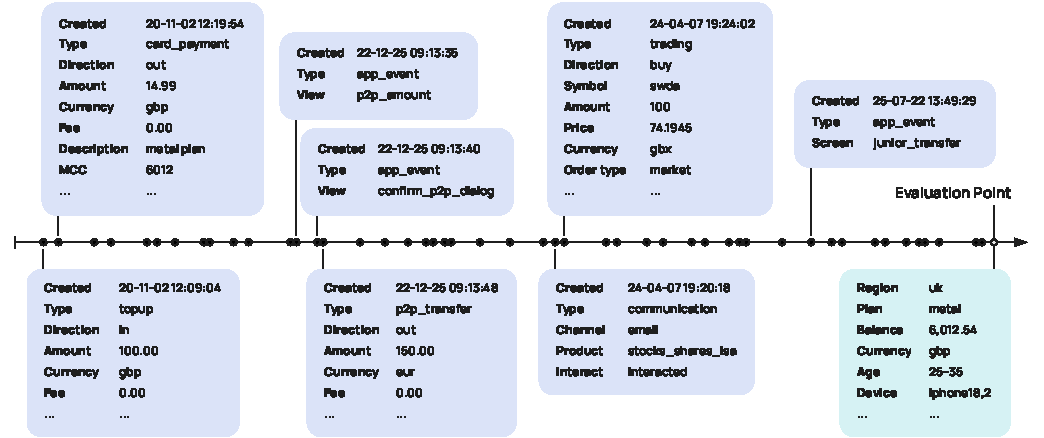
\includegraphics[width=1\linewidth]{images/timeline.pdf}
    \caption{
        \textbf{이벤트 타임라인 개요}.
        계정이 생성된 이후, 사용자들은 시간이 흐르며 거래, 인앱 내비게이션, 커뮤니케이션 등 플랫폼 상호작용 시퀀스를 만들어낸다.
        저자들은 지정된 평가 시점까지의 이벤트 이력을 모은다.
        이런 순차적 이벤트 외에, 그 시점에서의 레코드 상태를 기술하는 맥락 속성(예: 멤버십 플랜이나 서비스 지역)도 함께 담는다.
        이벤트와 속성 모두 동일한 표현을 공유한다 — 타임스탬프와 키--값 쌍 집합(예: \texttt{Type:} \texttt{card\_payment}, \texttt{Channel:} \texttt{email})이다.
        그림에 표시된 모든 값은 합성 데이터이며 예시일 뿐이다.
    }
    \label{fig:timeline}
\end{figure}

본 연구에서 사용된 모든 데이터는 완전 익명화되어 있으며 개인 식별 정보를 포함하지 않는다.
저자들은 사전학습 데이터셋을 111개국에 걸친 26\,M 사용자 레코드로 구성하며, 이는 24\,B 이벤트와 207\,B 토큰을 누적한다.

\subsubsection{이벤트 이력}
표준 플랫폼 사용은 계정 충전, 결제, 인앱 내비게이션, 서비스 커뮤니케이션 등 다양한 서비스에 걸쳐 이벤트 스트림을 생성한다.
이렇게 집계된 이벤트 이력은 다양한 분석·예측 과제를 뒷받침할 수 있는 인구 수준 패턴을 담아낸다.
하나의 이벤트는 생성 타임스탬프와 키--값 쌍 집합으로 정의된다(예: \texttt{Direction:} \texttt{out}).
저자들은 거래(transactions), 앱(app), 트레이딩(trading), 커뮤니케이션(communication)으로 느슨하게 묶을 수 있는 폭넓은 소스 타입에서 이벤트를 가져오며, 이들은 다운스트림 과제에 미칠 기대 영향이 큰 것을 기준으로 선정되었다.
이벤트 스키마는 소스 타입별로 다르며 서로 다른 키 집합을 갖는다(예: \texttt{Symbol} 키는 트레이딩 이벤트에만 있다).
익명화·비식별화와 표준 자격 기준 외에는, 운영 환경에서 발견되는 이질성을 모델이 온전히 포착할 수 있도록 이상치 제거나 어휘 가지치기 같은 추가적인 통계 필터링이나 전처리를 이벤트 스트림에 적용하지 않는다.

\subsubsection{프로필 상태}
이벤트 이력에 더해, 저자들은 잔고 분위(balance quantile), 플랜, 보험 상태, 서비스 지역 등 일반적인 맥락 속성을 함께 포함한다.
이 속성들은 이벤트 이력만으로는 빠지기 쉬운 유용한 맥락을 제공한다.
프로필 상태는 이벤트와 비슷한 형식의 기술적 키--값 쌍 집합이며(예: \texttt{Plan:} \texttt{metal}), 지정된 평가 시점(또는 사전학습에서는 컷오프 날짜)으로 타임스탬프가 찍힌다.

활동량이 매우 큰 사용자는 흔히 수만 건의 상호작용을 만들어내 계산 자원의 한계를 넘어선다. 저자들은 이를 고정 컨텍스트 창으로 잘라내어(truncation) 처리한다~(\S\ref{sec:training}).
그러나 이런 절단은 계정 연령처럼 유용한 신호를 담은 초기 역사적 이정표(milestone)를 잘라낼 위험이 있다.
이를 보완하기 위해 저자들은 프로필 상태에 \emph{라이프롱 이벤트(life-long events)} 를 덧붙인다. 일반 프로필 속성과 달리, 이 키--값 쌍들은 각각 최초 발생 시각을 기록하는 개별 타임스탬프를 갖는다(예: \texttt{Lifelong:} \texttt{first\_topup} at \texttt{20-11-02 12:09:04}).
이 타임스탬프는 평가 시점까지의 시간 거리를 계산하는 데 쓰이며, 모델이 역사적 이정표의 시점 정보를 인코딩할 수 있게 해 준다.

\subsubsection{사전학습 시간 범위}
견고하고 일반화되는 모델을 만들려면 역사적 커버리지를 극대화하는 것과 데이터의 관련성(relevance)을 유지하는 것 사이에서 섬세한 균형이 필요하다.
즉, 사전학습에 쓸 최적 시간 범위를 결정하는 일은 이벤트 다양성, 분포 변화(distribution shift), 계산 효율성 사이의 여러 트레이드오프를 풀어내는 작업이다.

첫째, 사용 가능한 전체 데이터셋의 모든 이벤트를 그대로 포함하는 것은 비실용적이며 최적이 아닌 경우가 많다.
오래된 이벤트는 추론 시점에는 더 이상 유효하지 않은 과거 패턴, 상품 기능, 시스템 동역학을 반영할 수 있다.
이런 불일치는 분포 어긋남(distribution mismatch)을 만들어내고, 결과적으로 진부한 과거 사례에서 배포 환경의 진화하는 행동 양상으로 일반화하기 어렵게 만든다.
또한 매우 긴 시간 범위에서 매우 이질적인 이벤트를 포함시키면 사전학습 과제 자체가 어려워지고 수렴이 느려질 수 있다.
둘째, 다운스트림 응용은 사전학습에 사용된 범위보다 훨씬 이전 또는 훨씬 이후 시점에 발생한 이벤트에 대해 예측해야 할 수 있다.
모델이 최근 패턴과 덜 흔한 과거 패턴 양쪽 모두에서 충분한 다양성을 보지 못했다면, 이런 분포 외 입력에서 성능이 떨어질 수 있다.
마지막으로, 트랜스포머 아키텍처의 유효 컨텍스트 길이는 모델 설계와 하드웨어 제약에 의해 제한된다.

이런 점들을 종합해, 저자들은 사전학습용으로 2023년부터 2025년에 걸친 25개월 시간 범위를 선택하며, 이는 충분한 이벤트 커버리지, 최근성, 분포 일관성, 그리고 다룰 수 있는 시퀀스 모델링 사이의 균형을 맞춘 것이다.
